\chapter{Проектирование корпуса}

Для перехода к корпусному виду сменим вид разьёма и поменяем под него форму платы (Рис~\ref{fig:BordShape}). Ширина убираемого зазора равна 1~мм

\begin{figure}[H]
	\centering
	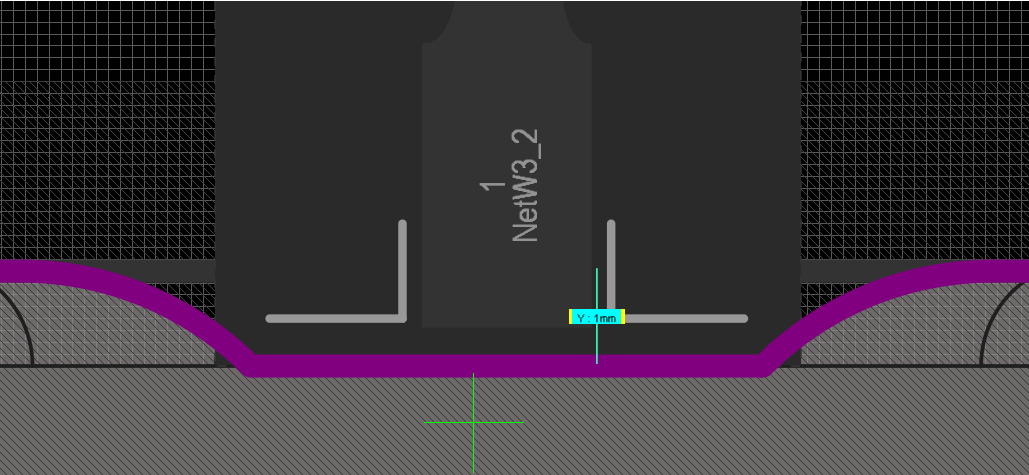
\includegraphics[width=0.8\textwidth]{BordShape.png}
	\caption{Размеры выступа.}%
	\label{fig:BordShape}
\end{figure}

Сделаем небольшие наброски для размеров ячеек. 
Граница корпуса будет описана в слое Mechanical~18. Набросочные границы ячеек — в слое Mechanical~20.

Аппроксимацию ячеек будем проводить прямоугольниками, при этом будем считать, что реальные ячейки будут вырезаться фрезой радиусом 2~мм, а следовательно от границы рамки до элемента должно быть не менее 2~мм.

Для расчёта максимального размера ячеек воспользуемся формулой
\[b[\text{мм}]\leq150/f_{max}[\text{ГГц}]\]
где  b  ---  максимальный  линейный  размер  ячейки,  мм, $f_{max}$ ---  максимальная возможная частота рабочего сигнала, ГГц.

При этом достаточно будет экранировать только ВЧ тракт, так как остальная схема достаточно защищена от паразитных илучений из-за \sout{стукачества, лол} экранирования отверстиями. 

После первой попытки осознаем, что плату необходимо удлинить на 1~см. Но нет худа без добра, и зато теперь  мы можем убрать столько же с боковой стороны.

Для удобства переместим точку 0 в первое монтажное отверстие.
По итогу получаем вот такой набросок:
\begin{figure}[H]
	\centering
	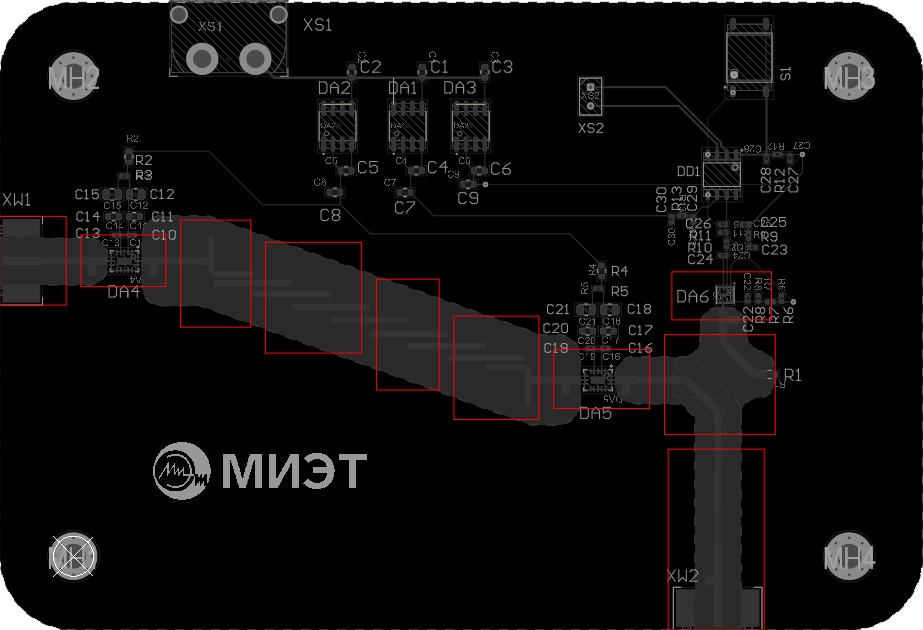
\includegraphics[width=0.7\textwidth]{CellsDraft.png}
	\caption{Предварительные ячейки.}%
	\label{fig:CellsDraft}
\end{figure}

Импортируем слои с границей платы, границами элементов и полосков и наброском ячеек в SolidWorks:
\begin{figure}[H]
	\centering
	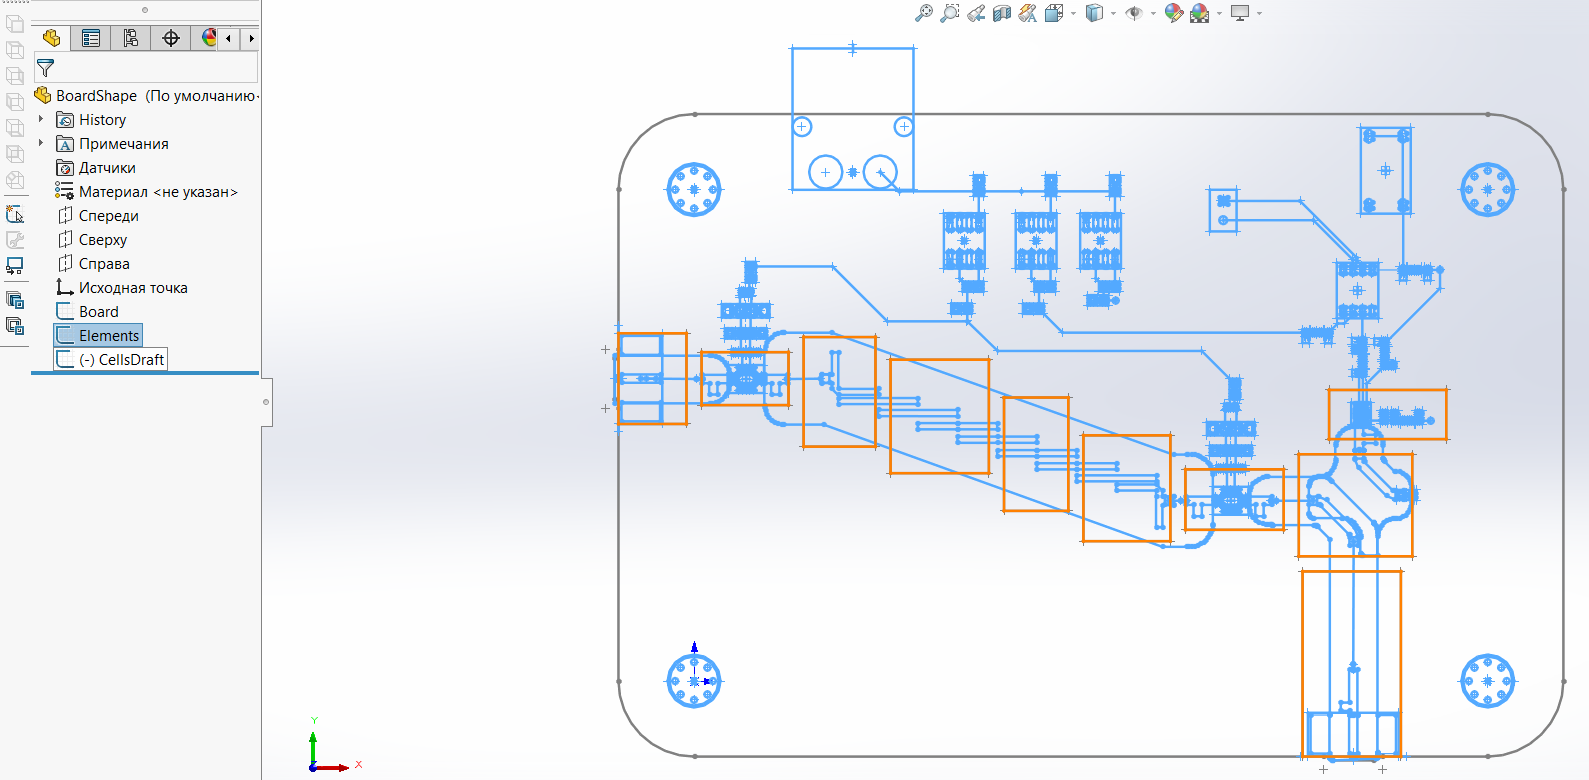
\includegraphics[width=0.8\textwidth]{BoardSolidDraft.png}
	\caption{Импортированные эскизы.}%
	\label{fig:BoardSolidDraft}
\end{figure}

Перерисуем (или переопределим размеры и привязки) для слоя ячеек, добавим крепёжные отверстия, прорубим ходы для линий и...  представляю вашему вниманию план побега Энди Дюфрейна:
\begin{figure}[H]
	\centering
	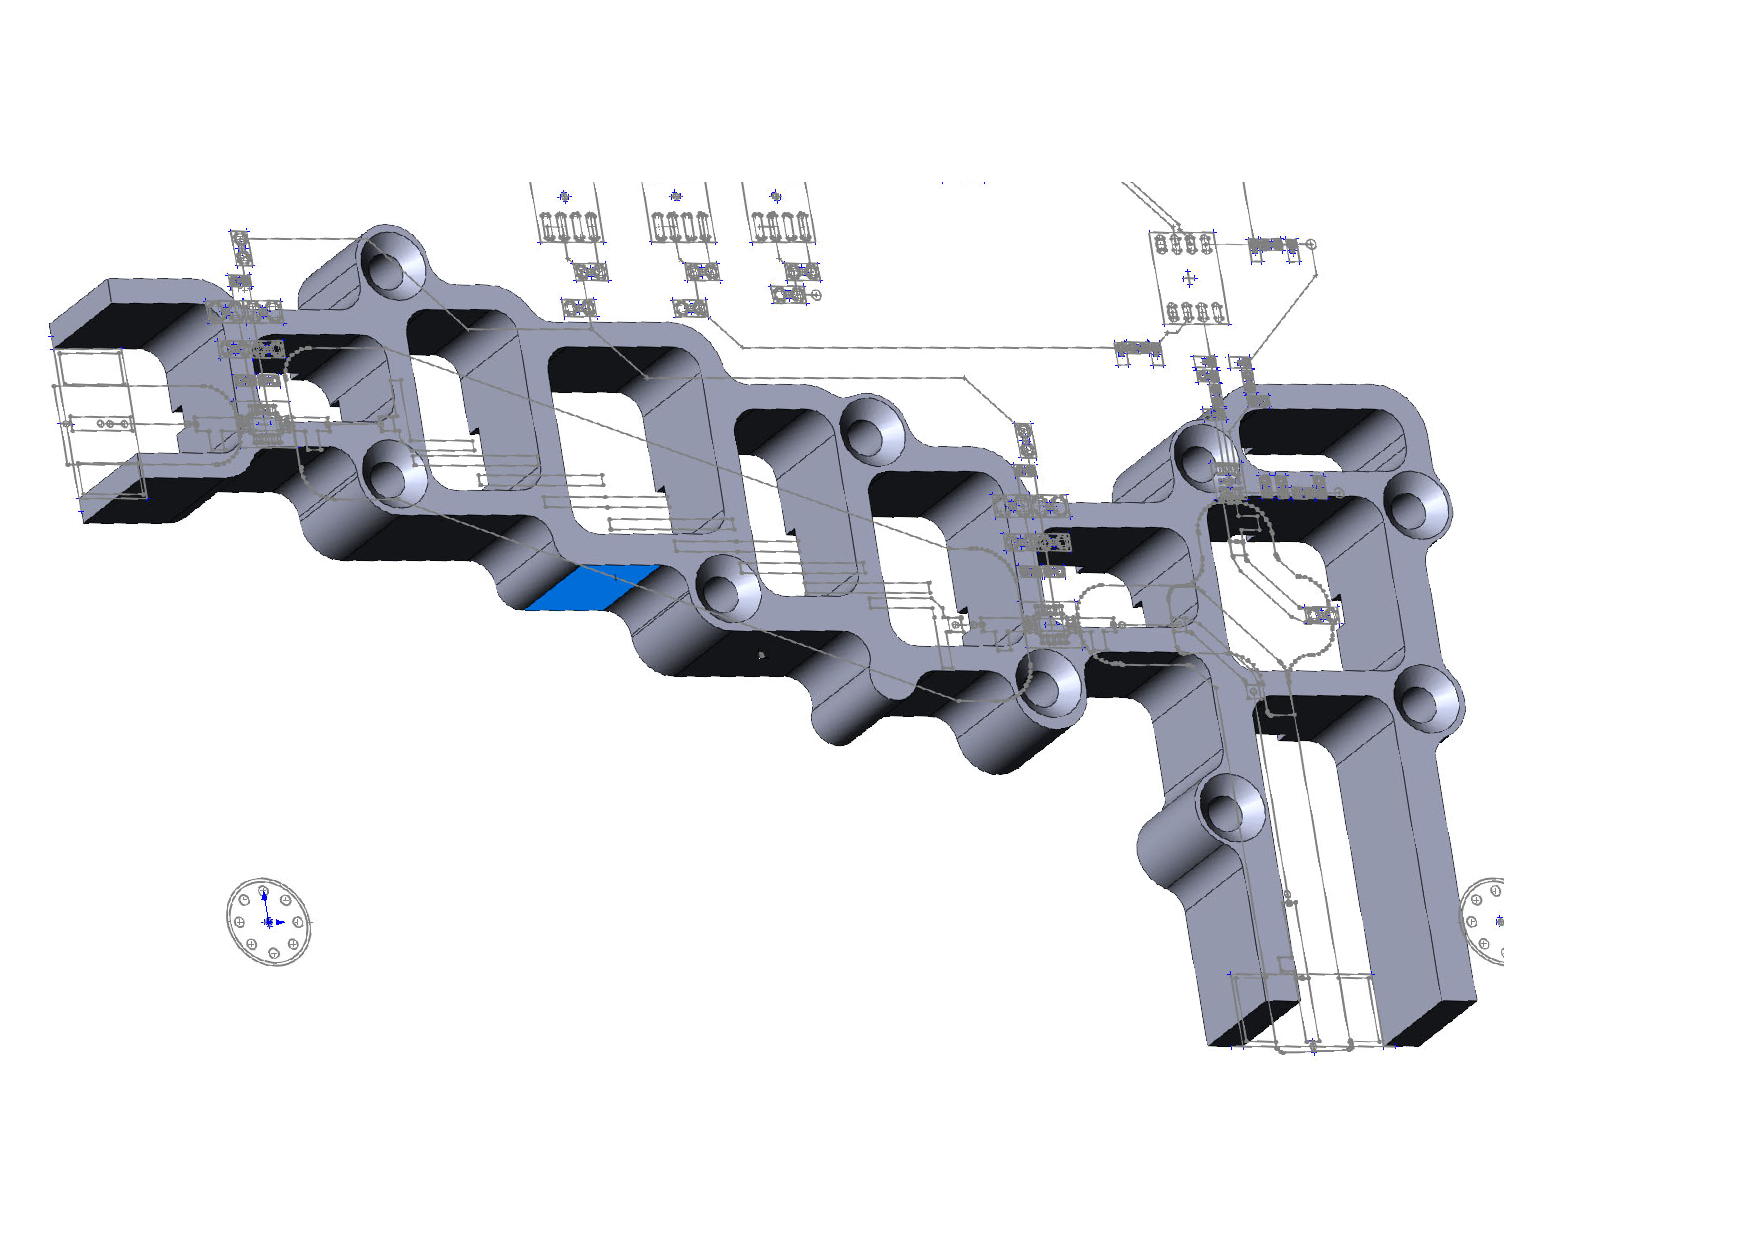
\includegraphics[width=0.8\textwidth]{CellsCutout.pdf}
	\caption{Ячеистая рамка.}%
	\label{fig:CellsCutout}
\end{figure} 

Экспортируем контур платы в DXF, добавим внешний контур так, чтобы стенка получилась 3 мм толщиной, добавим угловые крепёжные отверстия и получим корпус устройства.

\begin{figure}[H]
	\centering
	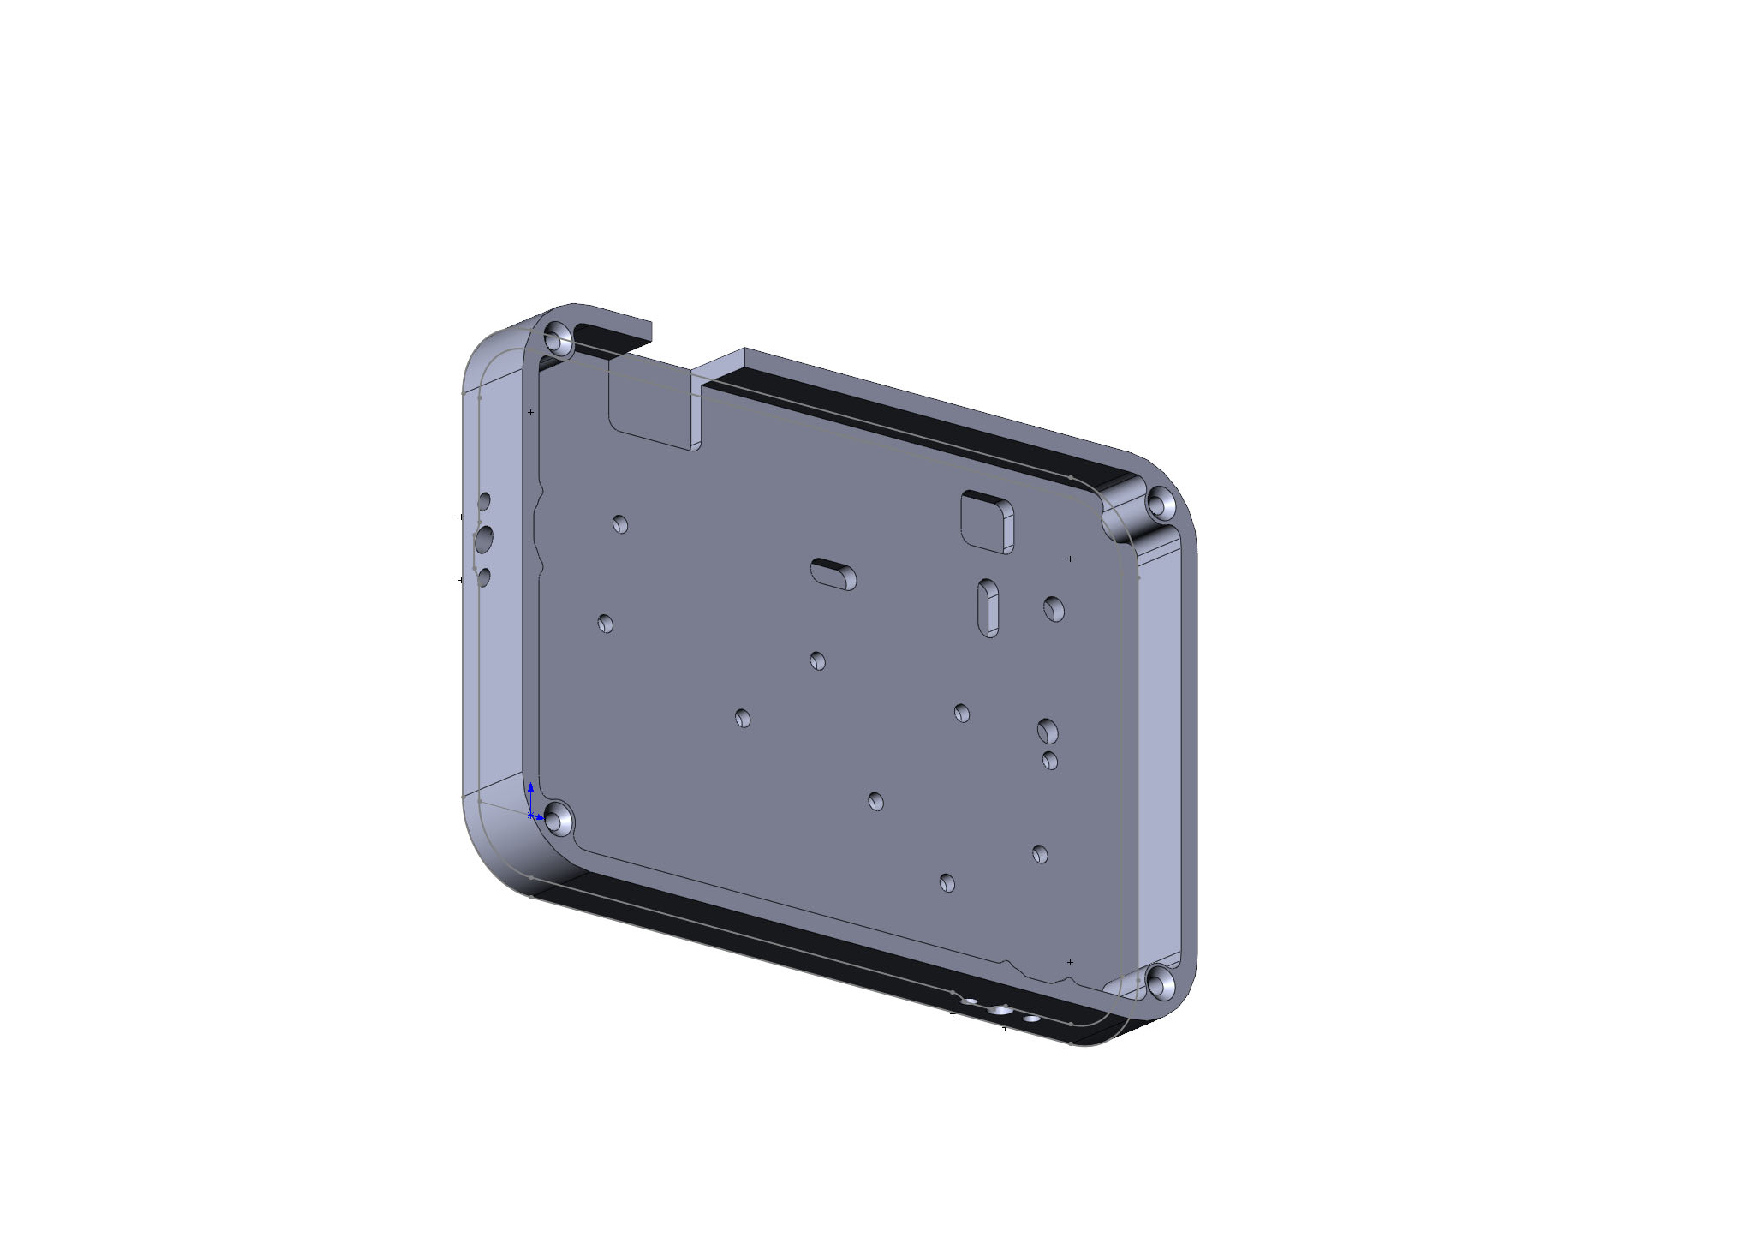
\includegraphics[width=0.6\textwidth]{BoardCase.pdf}
	\caption{Люлька нашего младенца.}%
	\label{fig:BoardCase}
\end{figure} 

Теперь спроектируем крышку и посмотрим, что у нас по итогу получилось:

\begin{figure}[H]
	\centering
	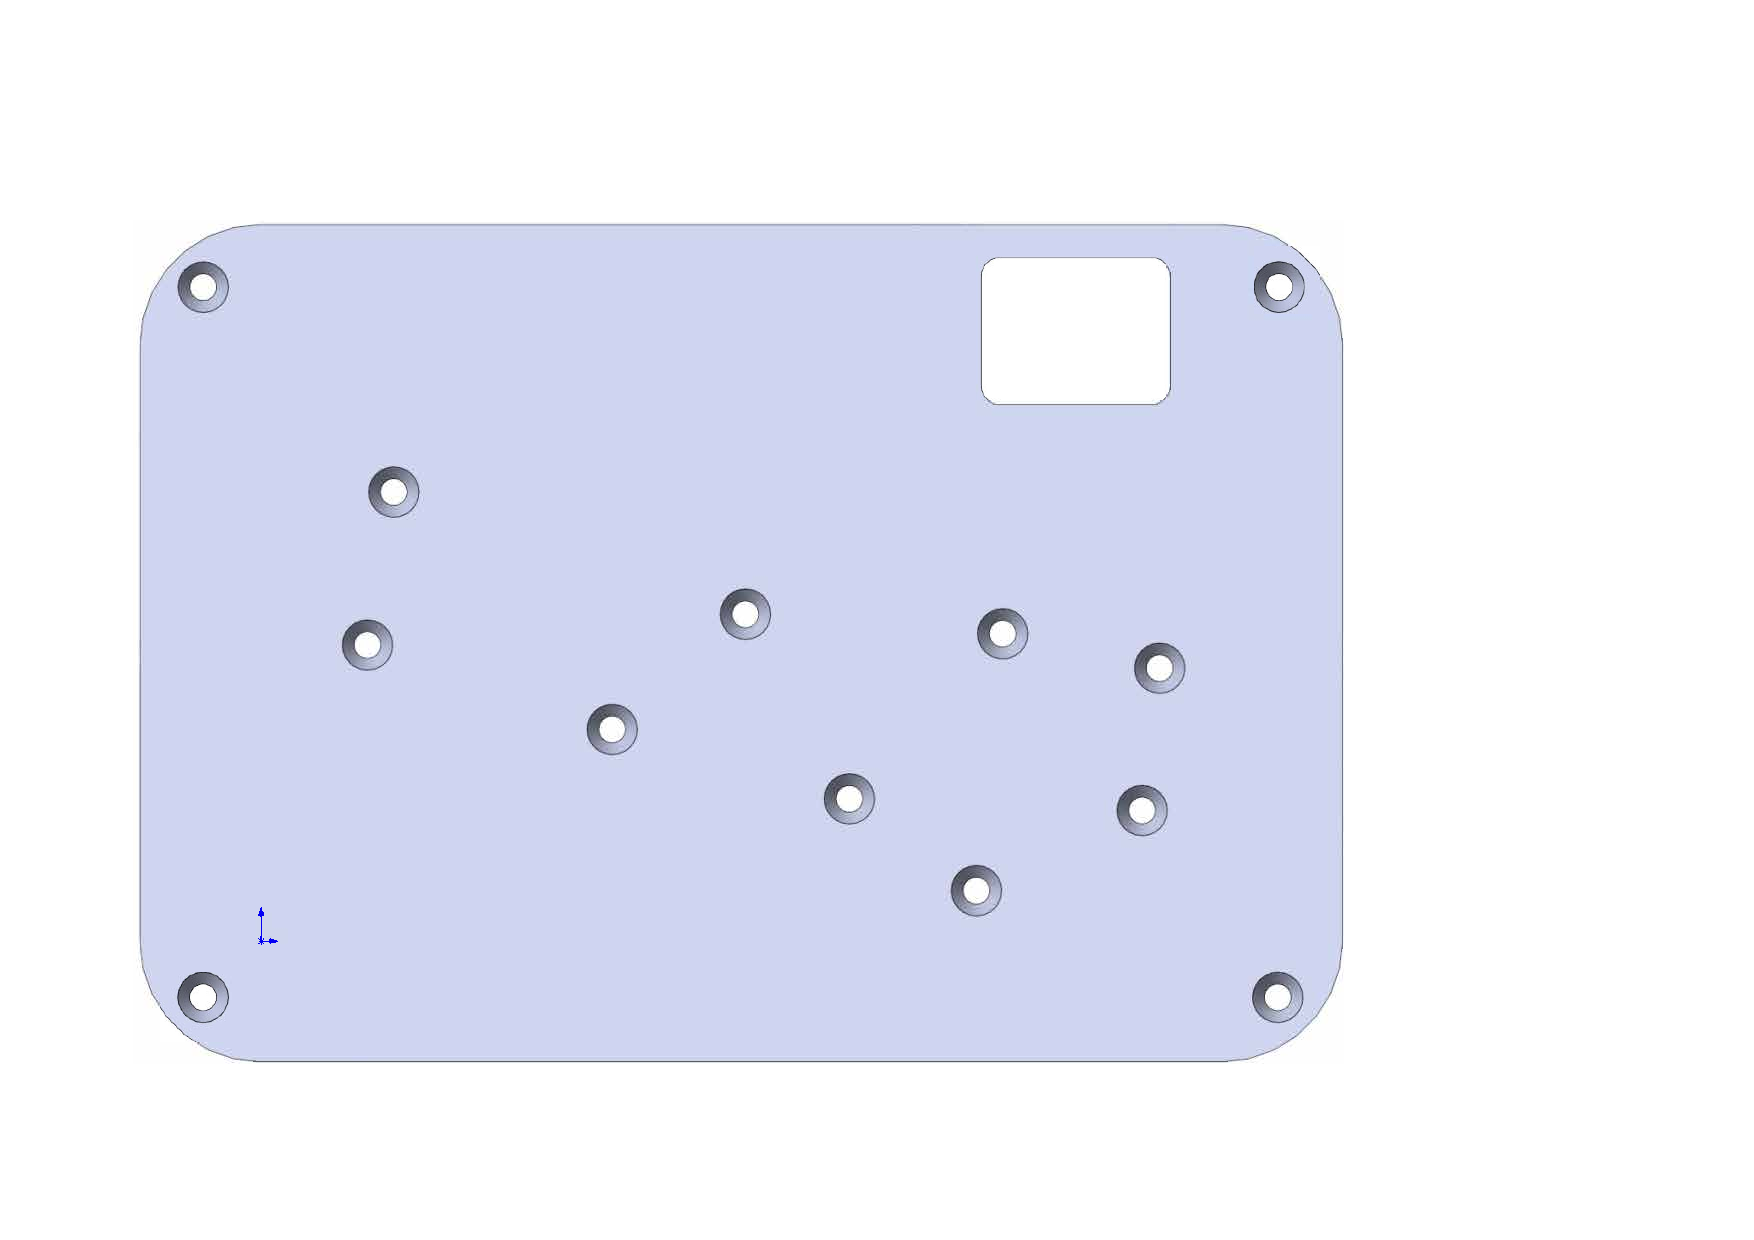
\includegraphics[width=0.6\textwidth]{BoardCup.pdf}
	\caption{Крышка изделия.}%
	\label{fig:BoardCup}
\end{figure} 

\begin{figure}[H]
	\centering
	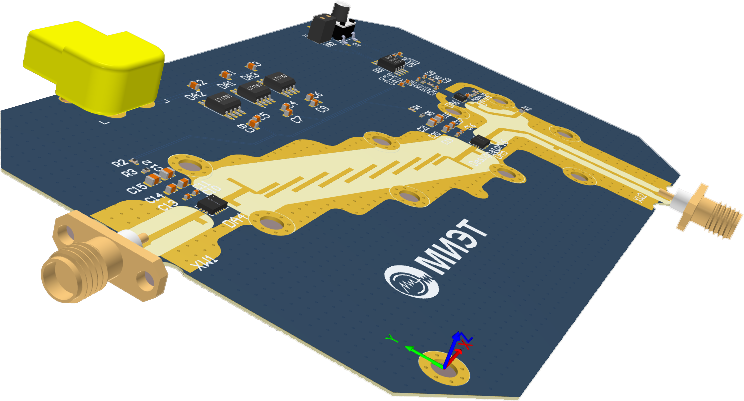
\includegraphics[width=0.6\textwidth]{OpenBoardRelease.png}
	\caption{Итоговый вид платы без корпуса}%
	\label{fig:OpenBoardRelease}
\end{figure} 

\begin{figure}[H]
	\centering
	\begin{subfigure}[b]{0.45\textwidth}
		\centering
		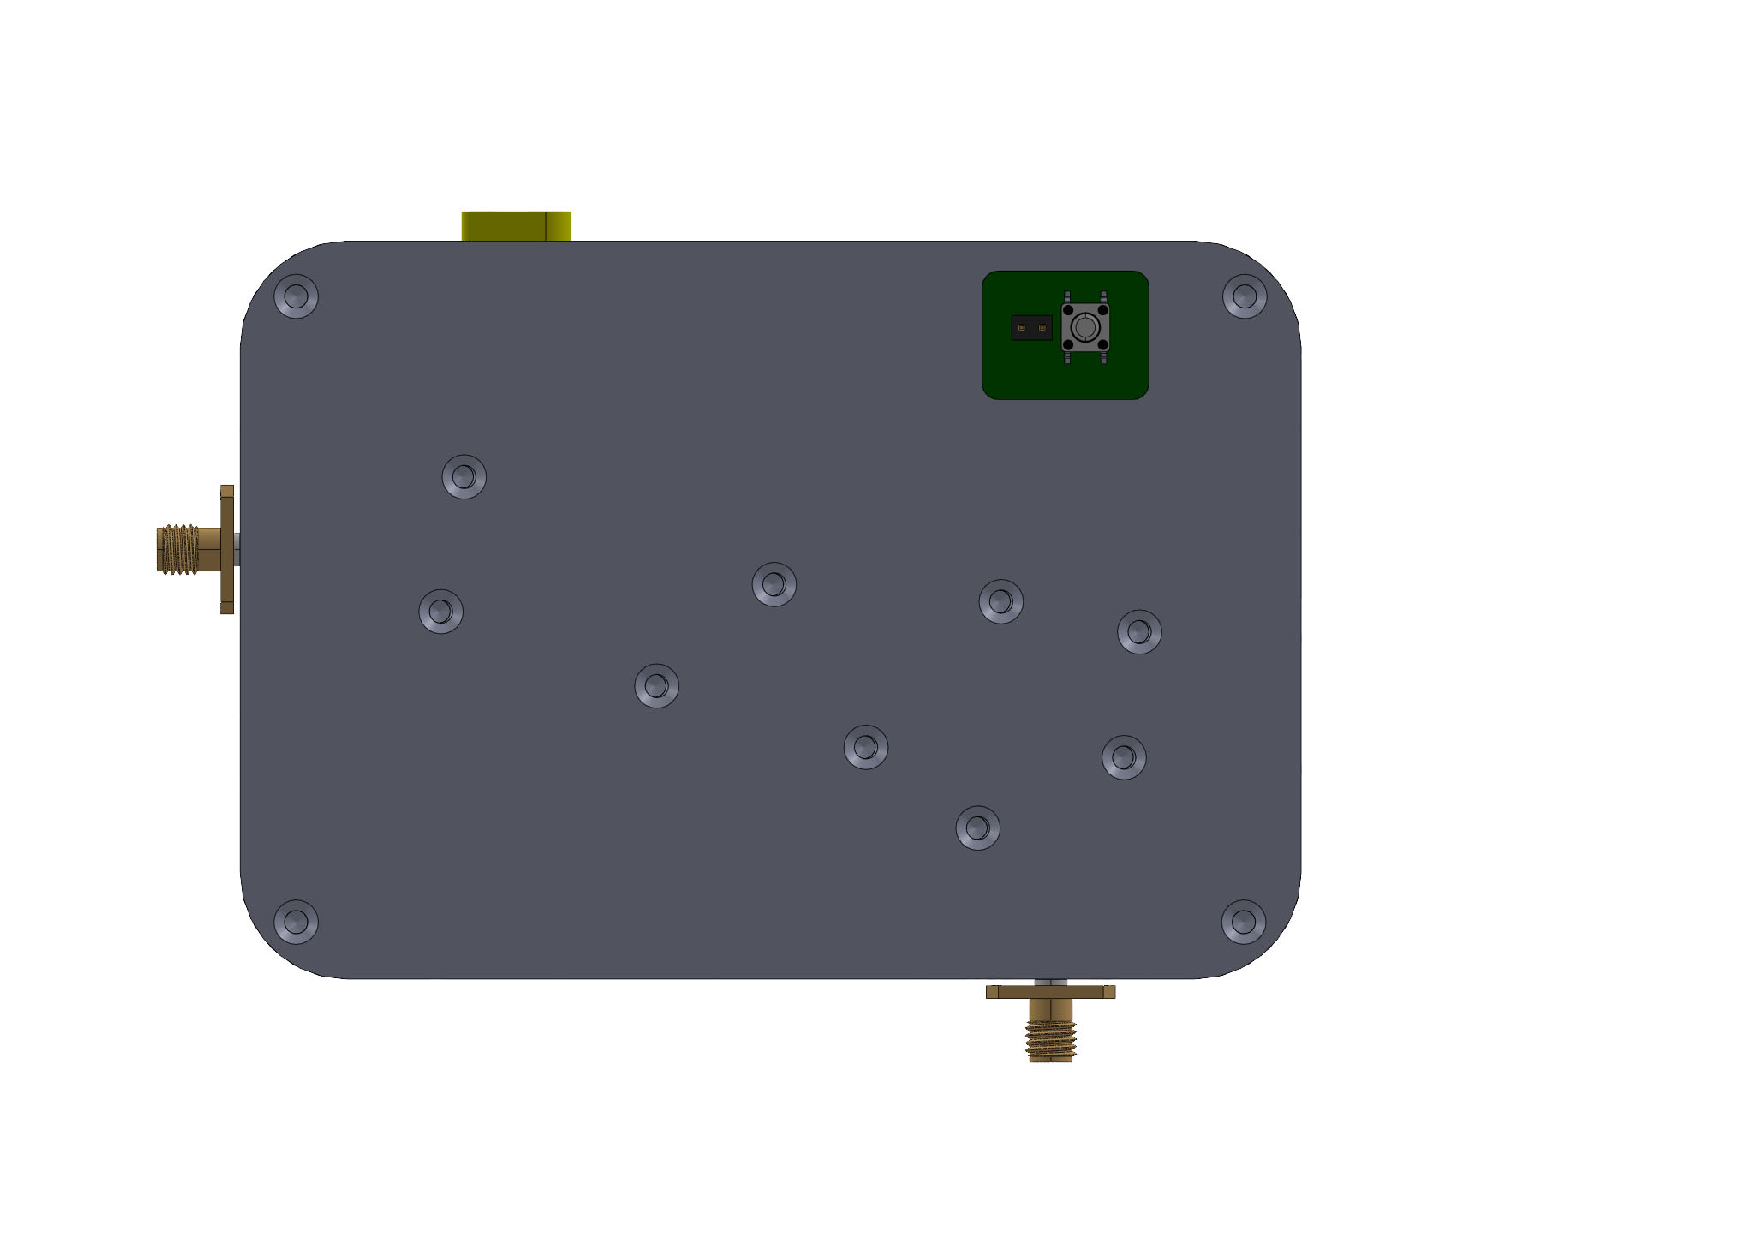
\includegraphics[width=\textwidth]{ShieldedBoardRelease}
		\caption{}%
		\label{fig:SolidMech}
	\end{subfigure}
	\hfill
	\begin{subfigure}[b]{0.45\textwidth}
		\centering
		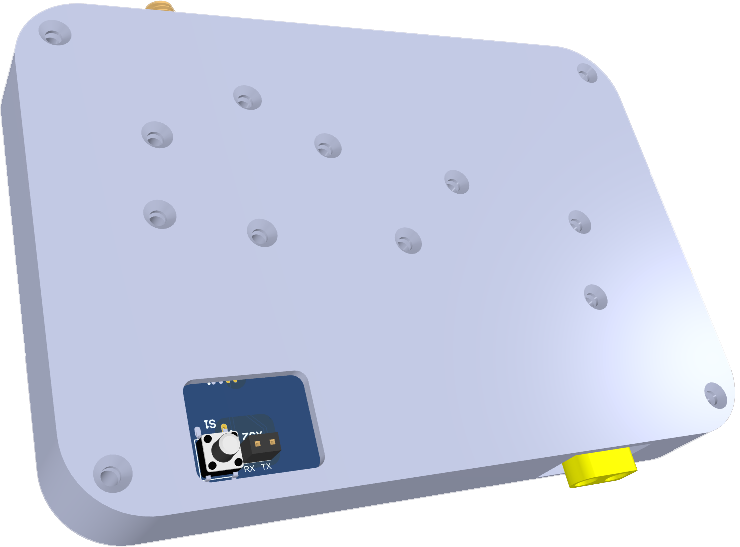
\includegraphics[width=\textwidth]{ShieldedBoardAltiumRelease.png}
		\caption{}%
		\label{fig:AltMech}
	\end{subfigure}
	\caption{%
		Графика ДМ
		(а) Вид модели в SolidWorks;
		(б) Вид модели в Altium 3D Viewer.
	}%
	\label{fig:MechanicalRelease}
\end{figure}

